\documentclass[11 pt]{article}

\usepackage{graphicx}

\usepackage{setspace}
\setstretch{1.25}

\begin{document}  
  \begin{titlepage}
\begin{center}
\huge{\bfseries{System Testing:}}\\
[2mm]
\huge{\bfseries{Prime Number Function}}\\
Version 1.0\\
  \vskip 0.2in
 Prince Ngema (754774)\\
 Tholithemba Mngomezulu (1512124)\\
 Luyanda Makhoba (834867) \\
 Takatso Molekane (569869)\\
 
 

\end{center}
 \end{titlepage}
 \tableofcontents
 \newpage
 \section{Purpose}
Ensuring that a system's faults have been eradicated is of most importance and this document describes how we have gone about the process of inspecting the PrimeNumbers function.
\section{Test Program Description}
The test program has been designed to detect and elliminate all possible bugs in the system. This has been achieved by listing all possible input variable types,both valid and invalid tests were conducted using exhaustive input testing tyes. Appropriate Error codes are returned for invalid input. Results of these tests were tabulated as comparisons were made with the expected results and simualtion results were recorded.\\



\subsection{Modification to parameters passed}
\begin{itemize}
\item
\textbf{Invalid parameters:}
\begin{itemize}
\item
String of characters
\item
Negative integers
\end{itemize}

\item
\textbf{Valid parameters:}
\begin{itemize}
\item
Numbers that can be stored as long
\item
 positive Integers
\end{itemize}
\end{itemize}

\section{Program Module Testing}
\subsection{Unit Tesing}
Testing of individual components using white-box method to evaluate all units of code in the program.\\
\newpage

Floor of testing events
\begin{figure}[h]
    \centering
    
    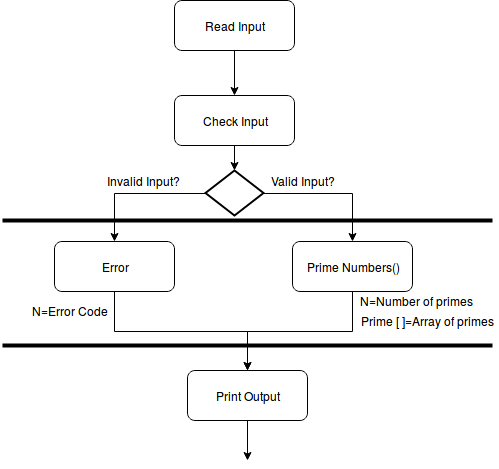
\includegraphics[width=\linewidth]{Integration Testing.png}
    \end{figure}


\subsubsection{Screnarios tested and results}

\begin{tabular}{|p{4cm}|p{3cm}|p{4cm}|p{3cm}|}
\hline
\textbf{Test case description} &\textbf{Test Data} & \textbf{Expected Result} & \textbf{Actual Result}\\
\hline
 user inputs a positive value & x= 10 & 4 primes and 1 3 5 7 & pass\\
 \hline
user inputs a negative value  & x= -1 &  Negative Integer and  Error Code 101-Negative 	int. Enter positive int & pass \\
 \hline
user inputs a char value string & x = Hello &String of char and Error Code 102-String of     character.Enter positive int0
 & pass \\
 \hline
 \end{tabular}


\subsubsection{White-box Testing}
One approach used invloved using data break points to view the values of variables at different points of the code during iterations. Using an IDE such as Visual Studio one can track and see as soon as the content of a variable changes.

The internal structure of PrimeNumber()

\subsection{Integration Tesing}
Integration testing is a kind of testing that is done by integrating all the methods and checking their interaction, for example observing that one methods output is read accordingly as the input of the relavant methods.\\
In our program, we have defined a function that takes in the input and then validates it to check if it conforms. If the input is valid(Positive integer), it is then passed from the checkInput() model to the PrimeNumber() function. The PrimeNumber() method returns an output.
We also checked to see that all method calls happened correctly and they passed these tests.\\
A common issue with intergration testing involves database locking of data which was not a problem we encounterd.

\subsection{System Tesing}
Testing the overal program. Checks overall run-through of the system.
\subsubsection{Black Box (Functional) testing}
High level design done by independent testers.\\

    \begin{figure}[h]
    \centering
    
    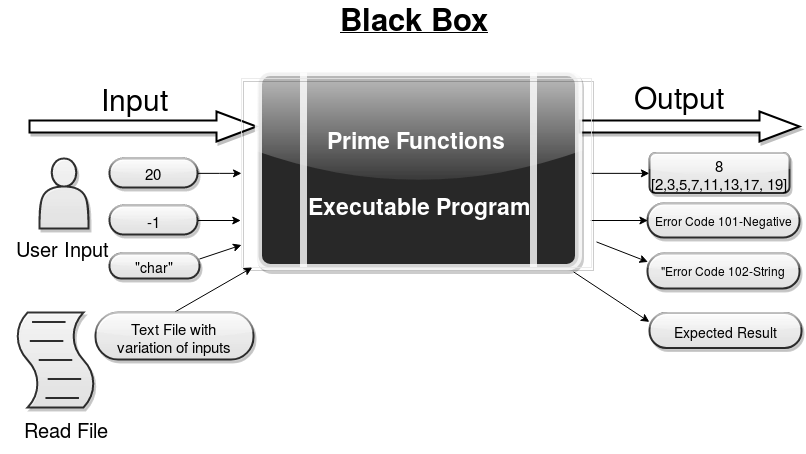
\includegraphics[width=\linewidth]{Black Box Diagram.png}
    \end{figure}
 

 \end{document}


